\section{Dise\~no de bajo nivel}
\label{lld}  
  \subsection{Paquetes y clases concretas}
  En esta secci\'on se presentan las clases concretas que implementan las
interfaces presentadas en la secci\'on~\ref{hld}. Para mayor claridad, se
dividieron los diagramas UML por paquetes.

  \subsubsection{Combinatory}   
    \begin{figure}
      \centering
      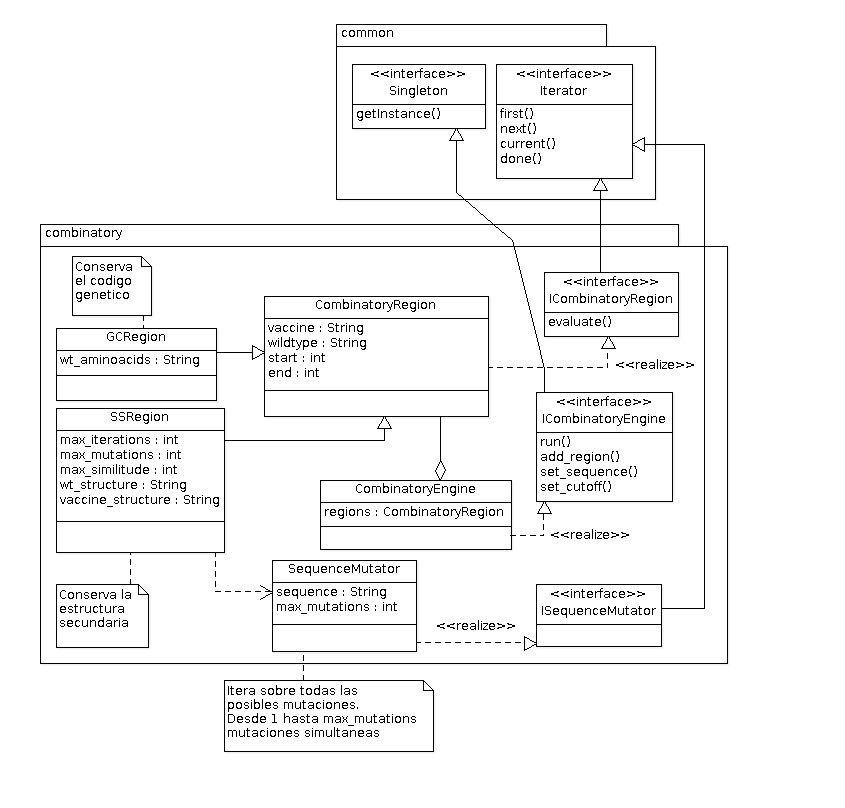
\includegraphics[scale=0.5]{lld-combinatory.png}  
      \caption{UML - Combinatory}
      \label{uml:lld-combinatory}
    \end{figure}

  En la Figura~\ref{uml:lld-combinatory} se puede ver el diagrama de clases
para el paquete \textit{combinatory}. Este paquete representa el componente
``CombinatoryEngine'' en la Figura~\ref{uml:architecture} de la
secci\'on~\ref{architecture}.

  La principal responsabilidad de este paquete es brindar al sistema, un motor
combinatorio de secuencias de ARN basado en restricciones. Para la primer
versi\'on de ``vac-o'' y seg\'un lo establece la especificaci\'on de
requerimientos, se contemplan dos tipos de restricciones.
  \begin{itemize}
   \item Conservaci\'on de la estructura secundaria (\textit{SSRegion}).
   \item Conservaci\'on del c\'odigo gen\'etico (\textit{GCRegion}).
  \end{itemize}

  El segundo caso, no merece mayor detalle a nivel de dise\~no. Por otro lado,
para la restricci\'on de conservar la estructura secundaria, vale la pena
profundizar en que implica garantizar esta responsabilidad.

  La clase \textit{SSRegion} es un \textit{iterator}, y los elementos sobre los
que debe iterar son aquellas secuencias de ARN que conservan una estructura
secundaria dada (\textit{vaccine\_structure}). Ya que la cantidad de secuencias
que conservan una misma estructura secundaria podr\'ia ser eventualmente muy
grande, se ofrecen dos restricciones complementarias para reducir el numero de
secuencias que son tenidas en cuenta. A continuaci\'on resumimos brevemente cada
una de estas restricciones:

  \begin{itemize}
   \item \textbf{Distancia m\'inima} a las secuencias que conservan una
estructura secundaria dada (\textit{wt\_structure}). Aquellas secuencias que
est\'en a menor distancia que la distancia m\'inima, ser\'an descartadas. La
cantidad de secuencias con las que se compara y calcula la distancia, lo
determina el valor de \textit{wt\_seq\_cache}.
  
  \item \textbf{Similitud estructural} a una estructura secundaria dada
(\textit{wt\_structure}). Esta restricci\'on implica un mayor costo
computacional ya que partiendo de una posible secuencia, se realizan desde una,
hasta \textit{max\_mutations} mutaciones simultaneas sobre toda la secuencia, y
para cada posible mutaci\'on, se comprara la estructura secundaria de la
mutaci\'on con la estructura \textit{wt\_structure}. Aquellas secuencias que
excedan el porcentaje \textit{max\_similitude} de similitud, ser\'an
descartadas.
  \end{itemize}

  \subsubsection{Validator}
    \begin{figure}
      \centering
      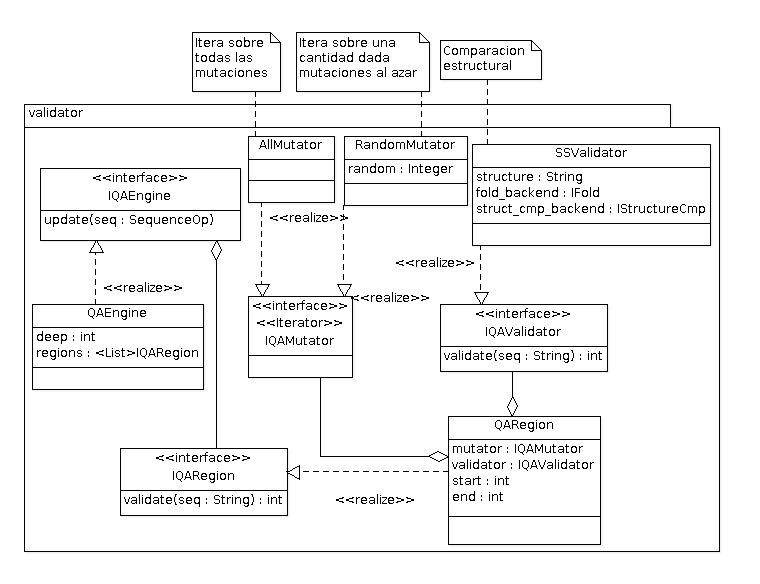
\includegraphics[scale=0.5]{lld-validator.png}  
      \caption{UML - Validator}
      \label{uml:lld-validator}
    \end{figure}

  En la Figura~\ref{uml:lld-validator} se puede ver el diagrama de clases
para el paquete \textit{validator}. Este paquete representa el componente
``QAEngine'' en la Figura~\ref{uml:architecture} de la
secci\'on~\ref{architecture}.

  La responsabilidad de este paquete es realizar una serie de pruebas que
garanticen al sistema que una secuencia dada, merece ser evaluada y tenida en
cuenta como posible optimizaci\'on de la vacuna. Las pruebas que se realizan
para garantizar la ``calidad'', se basan en que luego de sufrir alguna cantidad
acumulada de mutaciones, la secuencia mantenga determinadas propiedades en
determinadas regiones.

  En la primer versi\'on de ``vac-o'' se contemplan dos maneras de generar
mutaciones de una secuencia:
    \begin{itemize}
     \item Todas las mutaciones posibles (\textit{AllMutator})
     \item Una cantidad (\textit{random}) de mutaciones al azar
(\textit{RandomMutator})
    \end{itemize}
y dos propiedades a verificar sobre cada mutaci\'on:
    \begin{itemize}
     \item Comparaci\'on estructural con una estructura secundaria dada
(\textit{SSValidator}).
     \item Conteo y comparaci\'on de nucle\'otidos apareados o desapareados
(\textit{NUValidator}).
    \end{itemize}

  \subsubsection{LibRNA}
   \begin{figure}
      \centering
      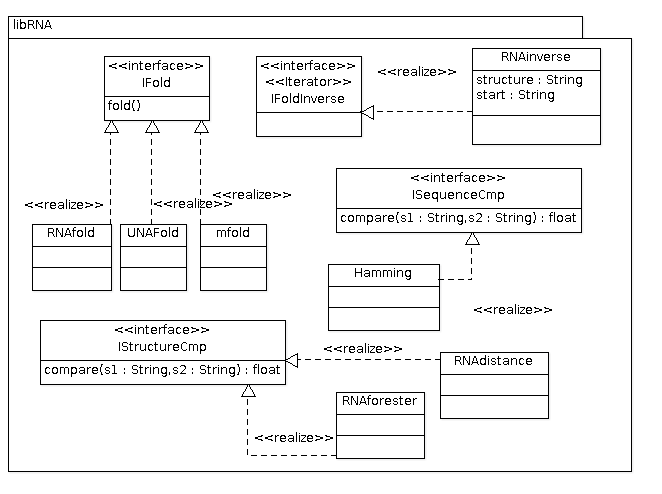
\includegraphics[scale=0.5]{lld-librna.png}  
      \caption{UML - LibRNA}
      \label{uml:lld-librna}
    \end{figure}

  En la Figura~\ref{uml:lld-librna} se puede ver el diagrama de clases
para el paquete \textit{libRNA}. Este paquete representa el componente
``libRNA'' en la Figura~\ref{uml:architecture} de la
secci\'on~\ref{architecture}.

  La responsabilidad de este paquete es brindar al sistema servicios para la
manipulaci\'on de secuencias de ARN. Para cumplir con esta responsabilidad, se
ofrece al sistema el acceso a librer\'ias externas de manera transparente y
permitiendo utilizar diferentes librer\'ias para acceder a diferentes servicios.

  En la primer versi\'on del sistema, se contemplan los siguientes servicios
como indispensables, aunque en futuras versiones se podr\'ian agregar otros:

  \begin{itemize}
   \item ``Folding'' directo (\textit{IFold})
   \item ``Folding'' inverso (\textit{IFoldInverse})
   \item Comparaci\'on entre estructuras (\textit{IStructureCmp})
   \item Comparaci\'on entre secuencias (\textit{ISequenceCmp})
  \end{itemize}

  La importancia de este paquete y las interfaces que contiene radica en que le
permite al resto del sistema, abstraerse del uso de una u otra librer\'ia, y
contar con una API unificada para acceder a estos servicios.    

  \subsubsection{Ranker}
  \begin{figure}
      \centering
      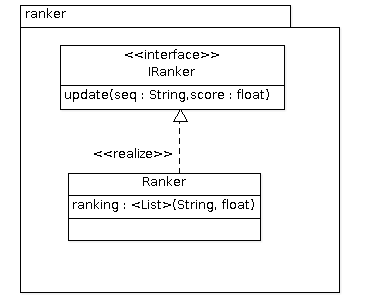
\includegraphics[scale=0.5]{lld-ranker.png}  
      \caption{UML - Ranker}
      \label{uml:lld-ranker}
    \end{figure}

  En la Figura~\ref{uml:lld-ranker} se puede ver el diagrama de clases
para el paquete \textit{ranker}. Este paquete representa el componente
``Ranker'' en la Figura~\ref{uml:architecture} de la
secci\'on~\ref{architecture}.

  \subsubsection{PluginAdmin}
  \begin{figure}
      \centering
      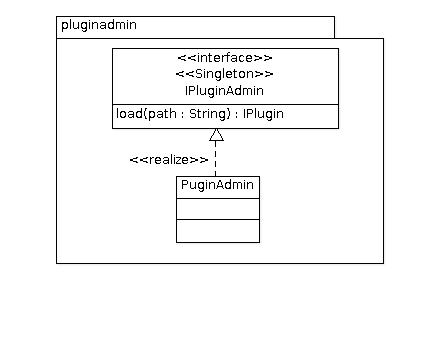
\includegraphics[scale=0.5]{lld-pluginadmin.png}  
      \caption{UML - PluginAdmin}
      \label{uml:lld-pluginadmin}
    \end{figure}

  En la Figura~\ref{uml:lld-pluginadmin} se puede ver el diagrama de clases
para el paquete \textit{pluginadmin}. Este paquete no aparece expl\'icitamente
en la arquitectura del sistema (Figura~\ref{uml:architecture} de la
secci\'on~\ref{architecture}), pero lo podemos identificar con la flecha que une
el componente ``Main'' con ``Plugin''.

  Fundamentalmente la responsabilidad de este paquete, es brindar al sistema la
funcionalidad de cargar las extensiones en memoria.

  \subsubsection{Plugin}
  Para el paquete \textit{plugin} no se especifica un dise\~no de bajo nivel
debido a que la implementaci\'on de cada extensi\'on no forma parte del sistema
``vac-o''. Simplemente, se asume que las extensiones que se implementen en el
futuro, deber\'an garantizar que cumplen con el ``contrato'' establecido por
las interfaces de este paquete.
